\documentclass[crop,tikz]{standalone}

\usepackage[utf8]{inputenc}
\usepackage{ifthen}
\usepackage{amsmath}

% 'crop' is the default for v1.0, before it was 'preview'
%\usetikzlibrary{...}% tikz package already loaded by 'tikz' option

\newcommand{\cross}[2]{

\begin{scope}[shift={#1}]
	\filldraw[black!30!white] (-#2,-#2) -- (-#2,-1) -- (#2,-1) -- (#2,-#2) -- (1,-#2) -- (1,#2) -- (#2,#2) -- (#2,1) -- (-#2,1) -- (-#2,#2) -- (-1,#2) -- (-1,-#2) -- cycle;
\end{scope}

}

\begin{document}

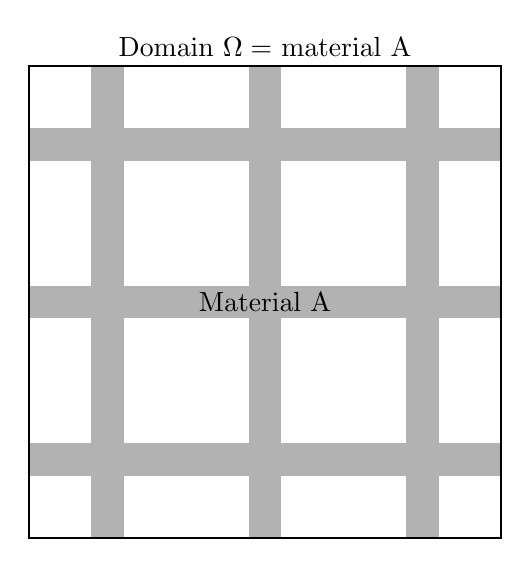
\begin{tikzpicture}

	\foreach \y in {0, ..., 1}
		\foreach \x in {0, ..., 1}
			\cross{(\x*2,\y*2)}{0.2}
			\cross{(-\x*2,-\y*2)}{0.2}
			\cross{(\x*2, -\y*2)}{0.2}
			\cross{(-\x*2,\y*2)}{0.2}
			; %end for \x
		; %end for \y
		
	\draw[thick] (-3,-3) rectangle (3,3);
	\node[anchor=south] at (0,3) {Domain $\Omega = $ material A};
	\node[align=center] at (0,0) {Material A};
		
\end{tikzpicture}

\end{document}